\chapter{Hierarchical Program Structures}

{
	\noindent
	\scshape\hfill\scriptsize Ole-Johan Dahl and C. A. R. Hoare\hfill
}
\renewcommand{\leftmark}{\normalfont\scriptsize\hfill OLE-JOHAN DAHL AND C. A. R. HOARE\hfill}

\section{Introduction}

In this monograph we shall explore certain ways of program structuring and point out their relationship to concept modeling.

We shall make use of the programming language SIMULA 67 with particular emphasis on structuring mechanisms. SIMULA 67 is based on ALGOL 60 and contains a slightly restricted and modified version of ALGOL 60 as a subset. Additional language features are motivated and explained informally when introduced. The student should have a good knowledge of ALGOL 60 and preferably be acquainted with list processing techniques.

For a full exposition of the SIMULA language we refer to the ``Simula 67 Common Base Language'' [\hyperref[ref:2]{2}]. Some of the linguistic mechanisms introduced in the monograph are currently outside the ``Common Base''\footnote{The Simula 67 language was originally designed at the Norwegian Computing Center, Oslo. The Common Base defines those language features which are common to all implementations. The Common Base is continually being maintained and revised by the ``Simula Standards Group'', each of whose members represents an organization responsible for an implementation. 8 organizations are currently represented on the SSG. (Summer 1971).}.

The monograph is an extension and reworking of a series of lectures given by Dahl at the NATO Summer School on Programming, Marktoberdorf 1970. Some of the added material is based on programming examples that have occurred elsewhere [\hyperref[ref:3]{3}, \hyperref[ref:4]{4}, \hyperref[ref:5]{5}].

\section{Preliminaries}

\subsection{Basic concepts}

Our subject matter as programmers is a special class of dynamic system, which we call computing processes or data processes. A programming language provides us with basic concepts and composition rules for constructing and analyzing computing processes.

The following are some of the basic concepts provided by ALGOL 60.

\begin{enumerate}[wide, nosep, label=(\arabic*)]
	\item A \textit{type} is a class of \textit{values}. Associated with each type there are a number of operations which apply to such values, e.g. arithmetic operations and relations for values of type \textbf{integer}.
	\item A \textit{variable} is a class of values of a given type ordered in a time sequence. The associated operations are accessing and assigning its current value. Both can be understood as \textit{copying} operations.
	\item An \textit{array} is a class of variables ordered in a spatial pattern. Associated is the operation of \textit{subscripting}.
\end{enumerate}

Notice that each of the concepts includes a data structure as well as one or more associated operations.

As another example consider machine level programming. The fundamental data structure is a bit string, which is not itself a very meaningful thing. However, combined with an appropriate sensing mechanism it has the significance of a sequence of Boolean values. In connection with a binary adder the bit string has the meaning of a number in some range, each bit being a digit in the base two number system. An output channel coupled to a line printer turns the bit string into a sequence of characters, and so forth. Thus the meaning of the data structure critically depends on the kind of operations associated with it.

On the other hand, no data process is conceivable which does not involve some data. In short, data and operations on data seem to be so closely connected in our minds, that it takes elements of both kinds to make up any concept useful for understanding computing processes.

\subsection{Higher level concepts}

As the result of the large capacity of computing instruments, we have to deal with computing processes of such complexity that they can hardly be constructed and understood in terms of basic general purpose concepts. The limit is set by the nature of our own intellect: precise thinking is possible only in terms of a \textit{small} number of elements at a time.

The only efficient way to deal with complicated systems is in a hierarchical fashion. The dynamic system is constructed and understood in terms of high level concepts, which are in turn constructed and understood in terms of lower level concepts, and so forth. This must be reflected in the \textit{structure} of the program which defines the dynamic system; in some way or another the higher level concepts will correspond to program components.

The construction of concepts suitable in a given situation is a creative process which often requires insights obtained at later stages of the system construction. Therefore, as programmers are painfully aware, any software project tends to be a complicated iterative process involving reconstruction and revision at each stage.

Each concept necessarily concerns a limited aspect of the system and
should correspond to a piece of program obtained by \textit{decomposition} of the total program. Good decomposition means that each component may be programmed independently and revised with no, or reasonably few, implications for the rest of the system. Thereby the total iteration process may be speeded up.

Any useful concept has some degree of generality, i.e. it is a class of
specialized instances. In other words one tries to group phenomena occurring in a dynamic system into \textit{classes} of phenomena and to describe each class by a single piece of program.

As an obvious example consider the arithmetic operations involved in a matrix multiplication. They may all be classified as dynamic instances (executions) of the single statement
$$
C[i, j] \coloneq C[i,j] + A[i, k] \times B[k, j];
$$

\noindent
provided that the matrix coefficients are classified as elements of two-dimensional arrays $A$, $B$, and $C$, and that the variables $i$, $j$, and $k$ are given values according to a certain pattern.

The above statement is not sufficiently well decomposed to be thought of as a ``concept''. The procedure declaration below, however, defines in a concise way the concept of matrix multiplication.

It is important that a concept may be classified as a \textit{syntactic category} (e.g. $\langle$block$\rangle$, $\langle$procedure$\rangle$) in a general language framework. Structured thought in terms of given concepts implies the construction of sentences, where the concepts have syntactic and semantic relationships to one another. The procedure below is related to other program components through calling sequences (procedure statements).

\quad \textbf{procedure} matmult$(A,\ B,\ C,\ m,\ n,\ p)$;

\quad \quad \textbf{array} $A$, $B$, $C$; integer $m$, $n$, $p$;

\quad \textbf{begin integer} $i$, $j$, $k$;

\quad \quad \textbf{for} $i\coloneq 1$ \textbf{step} 1 \textbf{until} $m$ \textbf{do}

\quad \quad \textbf{for} $j\coloneq 1$ \textbf{step} 1 \textbf{until} $n$ \textbf{do}

\quad \quad \textbf{begin} $C[i,\ j]\coloneq 0$;

\quad \quad \quad \textbf{for} $k\coloneq 1$ \textbf{step} 1 \textbf{until} $p$ \textbf{do}

\quad \quad \quad \quad $C[i,\ j]\coloneq C[i,\ j] + A[i,\ k] \times B[k,\ i]$

\quad \quad \textbf{end}

\quad \textbf{end};

The parameter mechanism of procedures in SIMULA deviates somewhat from that of ALGOL 60. The default transmission mode is by value for ordinary simple $\langle$type$\rangle$ parameters, and by ``reference'' for parameters of other kinds. This deviation is introduced for various pragmatic reasons, one of them being the compatibility with class declarations (cf. \ref{sec:frequency-histogram}). Thus, in the above procedure the parameters $i$, $j$, and $k$ are called by value, $A$, $B$, and $C$ by reference.

\subsection{Blocks and block instances}

One of the most powerful mechanisms for program structuring in ALGOL 60 is the block and procedure concept. It has the following useful properties from the standpoint of concept modeling.

\begin{enumerate}[wide, nosep, label=(\arabic*)]
	\item \textit{Duality}. A block head and block tail together define an entity which \textit{has properties} and \textit{performs actions}. Furthermore the properties may include a data structure as well as associated operators (local procedures).
	
	\item \textit{Decomposition}. A block where only local quantities are referenced is a completely self-contained program component, which will function as specified in any context. Through a procedure heading a block (procedure) instance may interact with a calling sequence. Procedures which reference or change non-local variables represent a partial decomposition of the total task, which is useful for direct interaction with the program environment.

	\item \textit{Class of instances}. In ALGOL 60 a sharp distinction is made between a block, which is a piece of program text, and a dynamic block instance, which is (a component of) a computing process. An immediate and useful consequence is that a block may be identified with the \textit{class} of its potential activation. (Strictly speaking a ``block'' in this context means either the outermost block or a block immediately enclosed by a dynamic block instance.) Through the recursion mechanism of ALGOL 60 different instances of the same block may co-exist in a computing process at the same time.

	\item \textit{Language element}. A block is itself a statement, which is a syntactic category of the language. Furthermore, through the procedure mechanism, reference to a block may be dissociated from its defining text.
\end{enumerate}

Referring back to our earlier discussion it appears that the ALGOL block mechanism has all the properties required of a concept modeling mechanism. On closer inspection, however, it turns out that the composition rules and interaction mechanisms provided place certain restrictions on the range of concepts to be formulated.

In ALGOL 60, the rules of the language have been carefully designed to ensure that the lifetimes of block instances are nested, in the sense that those instances that are latest activated are the first to go out of existence. It is this feature that permits an ALGOL 60 implementation to take advantage of a stack as a method of dynamic storage allocation and relinquishment. But it has the disadvantage that a program which creates a new block instance can never interact with it as an object which exists and has attributes, since it has disappeared by the time the calling program regains control. Thus the calling program can observe only the results of the actions of the procedures it calls. Consequently, the operational aspects of a block are overemphasized; and algorithms (for example, matrix multiplication) are the only concepts that can be modeled.

In SIMULA 67, a block instance is permitted to outlive its calling statement, and to remain in existence for as long as the program needs to refer to it. It may even outlive the block instance that called it into existence. As a consequence, it is no longer possible to administer storage allocation as a simple stack; a general garbage-collector, including a scan-mark operation, is required to detect and reclaim those areas of store (local workspace of block instances) which can no longer be referenced by the running program. The reason for accepting this extra complexity is that it permits a wider range of concepts to be conveniently expressed. In particular, it clarifies the relationship between data and the operations which may be performed upon it, in a way which is awkward or impossible in ALGOL 60.

\section[Object classes]{Object Classes}

A procedure which is capable of giving rise to block instances which survive its call will be known as a class; and the instances will be known as objects of that class. A class may be declared, with or without parameters, in exactly the same way as a procedure: 

\quad $\langle$class declaration$\rangle ::=$ \textbf{class} $\langle$class identifier$\rangle$

\tabto*{11.6em}$\langle$formal parameter part$\rangle$; $\langle$specification part$\rangle$;

\tabto*{11.6em}$\langle$class body$\rangle$

\quad $\langle$class body$\rangle ::= \langle$statement$\rangle$

Any variables or procedures declared local to the class body are called \textit{attributes} of that class; and so are the formal parameters, whether called by
value or called by reference. If the class body is not a block, it is regarded as if it were surrounded by block brackets \textbf{begin}\dots\textbf{end}.

A call of a class generates a new object of that class. The initial values of those of its attributes corresponding to formal parameters are specified in the actual parameter part of the generator. A generator always appears as a function designator, returning as its value a \textit{reference} to the newly generated object:

\quad $\langle$object generator$\rangle ::=$ \textbf{new} $\langle$class identifier$\rangle$

\tabto*{11.6em}$\langle$actual parameter part$\rangle$

In order to be able to refer again to a generated object, it is necessary to store the reference to it in a variable. Variables used for this purpose should be declared as of \textit{reference} type; and the declaration should also be \textit{qualified} by stating the class of objects to which that variable will refer.

\quad $\langle$reference variable declaration$\rangle ::=$ \textbf{ref} $(\langle $qualification$\rangle) \langle$identifier list$\rangle$

\quad $\langle$qualification$\rangle ::= \langle$class identifier$\rangle$

\noindent
The notation \textbf{ref} $(\langle$qualification$\rangle)$ may also be used to declare reference arrays, procedures, and parameters. An analogous mechanism for ``record handling'' was first proposed by Hoare [\hyperref[ref:6]{6}]. There is a neutral reference value none which does not refer to any object; and this is automatically assigned as initial value to every reference variable.

Reference values may be assigned, and tested for equality or inequality; but in SIMULA these operations are given special symbols, in order to emphasize the fact that they operate on references to objects, and not upon the current values contained in those objects.

\noindent
Thus:

\quad $:-$\tabto*{5.6em} denotes reference assignment

\quad $=\ =$\tabto*{5.6em} denotes reference equality

\quad $=/=$\tabto*{5.6em} denotes reference inequality.

\noindent
Reference values may also be passed as parameters, and they may be returned as the result of a function designator. A special example of such a function designator is of course the object generator which brings the object into existence, and passes back a reference to it as result.

\noindent
\textit{Example}:

\quad \textbf{class} $C(\dots)$; \dots class body for $C\dots$;

\quad \textbf{ref} $(C)X$;

\qquad \dots

\qquad \textbf{if} $X =\ =$ \textbf{none then} $X$: $-$ \textbf{new} $C(\dots)$;

The attributes of any object may be inspected or changed by the technique of \textit{remote identification}. If $X$ is a reference variable qualified by class $C$, and $A$ is an attribute identifier (i.e. local quantity) of that class, then $X.\,A$ refers to the attribute $A$ of the object currently referenced by $X$. If $X$ has the value \textbf{none}, the remote access is erroneous. If $A$ is a variable attribute, $X.\,A$ may appear to the left of an assignment, as an actual parameter, or in an expression. If $A$ is a procedure attribute, $X.\,A$ may appear as an actual parameter, or as a procedure statement or function designator, in which case it will be immediately followed by an actual parameter part. In short, a remote identifier $X.\,A$ may appear in any context in which an ordinary identifier may appear, except for a defining occurrence in a declaration.

In addition to reference variables, every reference parameter, function or expression has a qualification associated with it. In every assignment to a reference variable, it is possible to check that the assignment is valid, by comparing the qualifications of the left hand and right hand sides. SIMULA 67 has been designed to ensure that this check can be carried out wholly at compile time, thus avoiding the inefficiency of run-time checking, and the inconvenience of run-time error. Furthermore all remote identifiers can be checked at compile time to ensure that the combination of reference variable and attribute identifier is valid, so that the only error that has to be detected at run-time is when the reference variable has the value \textbf{none}.

The following sections provide examples of concepts modeled by means of class declarations.


\subsection{Frequency histogram}
\label{sec:frequency-histogram}

A frequency histogram of a real random variable with respect to given disjoint intervals can be represented by a table of integers $T_0, T_1, \dots, T_n$, where $T_i$ is the number of observations falling in the $i$th interval. A sequence of increasing numbers $X_1, X_2, \dots, X_n$ partitions the real axis into the following $n + 1$ intervals:
$$
\langle -\infty, X_1\rangle, (X_1, X_2\rangle, \dots, (X_n, \infty\rangle.
$$

\noindent
The $i$th relative frequency $(i = 0, 1, \dots, n)$ is equal to $T_i / N$, where $N$ is the total number of observations tabulated in the histogram.

We wish to represent the concept of a histogram as a self-contained piece of program, which can be incorporated in any subsequently written program which requires it. In a realistic program, it will be necessary to maintain several histograms to tabulate different random variables; for example, it may be necessary to record not only random lengths, but also random weights and random heights, and this will require three separate histograms, existing simultaneously with each other and with the main program which has generated them and which is using them. Furthermore, the numbers of the intervals and the partitioning values between them may be different in each case. This suggests that the histogram should be declared as a \textit{class}, with two parameters:

\quad \textbf{class} histogram$(X,\ n)$; \textbf{array} $X$; \textbf{integer} $n$;

where X is a real array of n elements specifying the boundaries of the partitions. The main program will use this class in the following way:

\quad \textbf{begin ref} $($histogram$)$ heights, weights, lengths;

\quad \quad \textbf{real array} $A[1:7]$, $B[1:12]$;

\quad \quad \dots initialise $A$, $B$\dots;

\quad \quad heights: $-$ \textbf{new} histogram$(A,\ 7)$;

\quad \quad weights: $-$ \textbf{new} histogram$(B,\ 12)$;

\quad \quad lengths: $-$ \textbf{new} histogram$(A,\ 7)$;

\quad \quad \dots rest of program\dots

\quad \textbf{end}

In the rest of the program, the three histograms may be referred to by the names of the three reference variables. In order to record each new observation (say $h$ or $w$) in the appropriate histogram, the program will contain the corresponding calls on a procedure tabulate:

\quad weights.tabulate$(w);$

\quad heights.tabulate$(h);$

The procedure ``tabulate'' must therefore be an attribute of the histogram class. Another attribute of the class must be the array $T$ which counts the number of observations in each interval; and also a variable $N$ to count the total number of observations recorded so far. Finally, a function frequency$(i)$ is required so that the relative frequency of observations in the $i$th interval may be read out. The only action required of the class body is to initialize these variables.

The declaration of the histogram class may be given:

\quad \textbf{class} histogram$(X,\ n)$; \textbf{array} $X$; \textbf{integer} $n$;

\quad \quad \textbf{begin integer} $N$; \textbf{integer array} $T[0:n]$;

\quad \quad \quad \textbf{procedure} tabulate$(Y)$; \textbf{real} $Y$;

\quad \quad \quad \quad \textbf{begin integer} $i$; $i\coloneq 0$;

\quad \quad \quad \quad \quad \textbf{while} (\textbf{if} $i < n$ \textbf{then} $Y < X[i + 1]$ \textbf{else false}$)$

\quad \quad \quad \quad \quad \quad \textbf{do} $i\coloneq i + 1$;

\quad \quad \quad \quad \quad $T[i] \coloneq T[i] + 1; N\coloneq N + 1$

\quad \quad \quad \quad \textbf{end} of tabulate;

\quad \quad \quad \textbf{real procedure} frequency$(i)$; \textbf{integer} $i$;

\quad \quad \quad \quad frequency $\coloneq T[i]/N$;

\quad \quad \quad \textbf{integer} i;

\quad \quad \quad \textbf{for} $i\coloneq 0$ \textbf{step} 1 \textbf{until} $n$ \textbf{do} $T[i]\coloneq 0;\ N\coloneq 0$

\quad \textbf{end} of histogram;

\textit{Note}. (1) In SIMULA 67, all simple parameters of a class or a procedure are called by value, even if the value parts are omitted. Arrays and other parameters are called by name.

(2) In SIMULA 67 all variables are automatically initialized on declaration to neutral values, \textbf{false} for Booleans, 0 for numbers, \textbf{none} for references. Thus in the examples given above the statements $i\coloneq 0,\ N\coloneq 0$, and the loop initializing $T$ could have been omitted.

It seems reasonable to claim that this piece of program adequately represents the concept of a histogram, in that it expresses the close relationship between the data items $X$, $n$, $T$ and $N$, and the operation of tabulation which
is to be performed on them. It would be possible, of course, to write the
operation in ALGOL 60 as a separate procedure with many parameters:

\quad \textbf{procedure} tabulate$(X,\ n,\ T,\ N,\ y)$;

\noindent
which records observation $y$ in the histogram $T$ in accordance with partitions defined by $X$, and also increments $N$. But this would be an artificial separation
of the operational aspect of the histogram from the data storage aspect; and the failure in adequately representing the concept is evidenced by the complexity of the specification of the procedure and the awkwardness of its use. 

It is worth while to explain the effect of creating a new object of class histogram by means of the statement

\quad weights: $-$ \textbf{new} histogram$(B,\ 12)$.

\noindent
First, a new object is created, consisting of the variables brought into existence by execution of the declarations for $T$, $N$, $i$, and the parameters $X$ and $n$, which are initialized to $B$ and 12 respectively. The body of the class declaration is now executed to initialize the other variables. On exit from the body, the variables are \textit{not} deallocated. Rather a reference (pointer, address) to them is passed back and assigned to the variable ``weights''. It is convenient to think of an object as a complete textual copy of the class body (including the specification part), in which the parameters and local variables and arrays correspond to actual storage locations. Thus an object may well contain local procedure (and even class $-$) declarations, as well as executable statements.

Subsequently, on execution of the procedure call weights. tabulate($w$), it is the tabulate procedure local to the object referenced by ``weights'' that is actually executed, and causes updating of the local attributes $T$ and $N$ of that object and no other.

\subsection{Gauss-integration}

A definite integral may be approximated by an ``$n$-point Gauss formula'', which is a weighted sum of $n$ function values computed at certain points in the integration interval.
$$
\int_a^b f(x)\text{d}x \approx \sum_{i = 1}^n w_i f(x_i)
$$

\noindent
The weights and abscissa values are chosen such as to give an exact result for the integral of any polynomial of degree less than $2n$. By a suitable transformation we find
$$
w_i = (b - a)W_i \quad\text{and}\quad x_i = a + (b - a)X_i,
$$

\noindent
where $W_i$ and $X_i(i = 1, 2, \dots, n)$ only depend on $n$, and not on $a$ or $b$. The idea of Gauss-integration is expressed in the following partly informal class declaration.

\quad \textbf{class} Gauss$(n)$; \textit{integer} $n$;

\quad \textbf{begin array} $W$, $X[1:n]$;

\quad \quad \textbf{real procedure} integral$(f,\ a,\ b)$;

\quad \quad \textbf{real procedure} $f$; \textbf{real} $a$, $b$;

\quad \quad integral $\coloneq \sum_{i=1}^n W[i] \times f(a + (b - a)\times X[i])\times (b- a)$;

\quad \quad compute $W[1], \dots, W[n], X[1], \dots, X[n]$ as

\quad \quad functions of $n$

\quad \textbf{end} of Gauss;

\quad \dots

\quad \textbf{ref} $($Gauss$)$ GS, G7;

\quad \dots

\quad GS: $-$ \textbf{new} Gauss$(S)$; G7: $-$ \textbf{new} Gauss$(7)$;

\quad \dots

\quad GS.integral$(F,\ A,\ B)$ \dots G7.integral$(F,\ A,\ B)$\dots

\noindent
\textit{Comments}. The variables GS and G7 refer to the concepts ``$S$-point'' and ``7-point Gauss-integration''. Each of them is a \textit{specialized instance} of the
more general concept of ``$n$-point Gauss-integration'', represented by the class.

A Gauss object computes once and for all the values of its local array elements, after which control returns to the $\langle$object generator$\rangle$. The procedure ``integral'' is intended for repeated use from outside the object.

The example indicates that the \textit{own}-concept of ALGOL is superfluous in this framework.

\section{Coroutines}

In ALGOL 60, a most powerful method of combining two pieces of program to accomplish some task is to declare one of them as a procedure, and to invoke it (possibly repeatedly) from within the other. However, in some cases the relationship between the two pieces of program is not fairly represented by this form of master$/$subordinate relationship; and it is better to regard them as \textit{coroutines} operating in some sense at the same level.

A simple example of coroutine structuring is provided by a games-playing program, which calculates its own move and outputs it to its opponent, inputs the opponent's response, computes its next move, and so on until the game is complete. Suppose now that two different programs have been constructed to play the same game, and it is desired to see which of them is the stronger player. The complete program to play the game is very naturally structured from its two component players, but the structuring method is that of the coroutine rather than the subroutine.

Another example of coroutine structuring is provided in a two-pass compiler for a programming language. The first pass normally outputs a long sequence of messages which are subsequently input by the second pass. However, if sufficient main storage is available to accommodate the program for both passes simultaneously, it is possible to arrange for the whole translation to be carried out apparently in a single pass, where the sequence of messages is transmitted \textit{piecewise} from the first pass to the second pass. First, the second pass is executed until it reaches its first request for an input message. The first pass program is then executed until it produces its first output message. The message is then handed over to the second pass, and the process is repeated until the second pass is complete. In some circumstances it might be possible to restructure one of the passes as a subroutine to the other; but since the choice would be arbitrary, it is better to regard the two programs as coroutines.

This case may be distinguished from the games-playing example in that the flow of information is in one direction only, from the first pass program which ``produces'' it to the second pass program which ``consumes'' it. This suggests that a single coroutine may profitably be regarded as a complete selfcontained program whose input and output instructions have been replaced by calls upon other coroutines to produce and consume the data. Each time a coroutine passes control to another coroutine for this purpose, it will expect to resume at the next following instruction. The instruction which causes transfer of control to another coroutine is known as

\quad resume$(X)$

\noindent
where $X$ refers to the coroutine being resumed.

In SIMULA, a coroutine is represented by an object of some class, cooperating by means of resume instructions with objects of the same or another class, which are named by means of reference variables. The communication of information may be accomplished in variables either global to all the objects or local to one of them; a producing coroutine assigns values to these variables, and the consuming coroutine accesses them. In the case of two-way communication, both coroutines may update the same global variables in turn.

When an object is first generated, it has a subordinate, procedurelike relationship to the block instance which generated it. This is evidenced by the fact that control automatically returns to the generator upon passage through the end of the object. The object does not in general know the identity of its generating block instance; it cannot therefore use a resume instruction to achieve the effect of a coroutine exit. A special, parameterless ``detach''' instruction is therefore provided by which a generated object can return control to the generator. The generator may then resume the detached object at the point following its (most recently executed) detach instruction by the
statement

\quad call$(X)$

\noindent
where $X$ is a reference to the detached object. Now the object is again in a subordinate position, with respect to the caller, and has an obligation to return to it either by a detach instruction or by going through its own \textbf{end}.

Thus a main program may establish a coroutine relationship with an object that it has generated, using the call/detach mechanism instead of the more symmetric resume$/$resume mechanism. In this case, the generated object remains subordinate to the main program, and for this reason is sometimes known as a \textit{semicoroutine}. But a semicoroutine may also be a full coroutine with respect to a group of other generated objects, with which it communicates by means of resume statements. In this case, if any of the group issues a detach, control returns to the master program which originally called a particular member of the group. Thus a coroutine issuing a resume statement imposes on the resumed coroutine its own responsibility, eventually to pass control back to the original caller by means of a detach.

Let $X$ and $Y$ be objects, generated by a ``master program'' $M$. Assume that M issues a call$(X)$, thereby invoking an ``active phase'' of $X$, terminated by a detach operation in $X$; and then issues a call$(Y)$, and so forth. In this way $M$ may act as a ``supervisor'' sequencing a pattern of active phases of $X$, $Y$, and other objects. Each object is a ``slave'', which responds with an active phase each time it is called for, whereas $M$ has the responsibility to define the large scale pattern of the entire computation.

\begin{figure}[h]
	\centering
	\includegraphics[width=.3\textwidth]{chap3/fig1}
\end{figure}

\noindent
Alternatively the decision making may be ``decentralised'', allowing an object itself to determine its dynamic successor by a resume operation.

\begin{figure}[h]
	\centering
	\includegraphics[width=.5\textwidth]{chap3/fig2}
\end{figure}

The operation resume$(Y)$, executed by $X$, combines an exit out of $X$ (by detach) and a subsequent call$(Y)$, thereby bypassing M. Obligation to 	return to $M$ is transferred to $Y$.

The history of a typical coroutine object may be summarized as follows:

\begin{enumerate}[wide, nosep, label=(\arabic*)]
	\item Upon generation, an object starts performing the operations of its class body, and is said to be \textit{operating} and \textit{attached} to (the block instance containing) the object generator which calls it into existence.
	\item The object issues a \textit{detach} statement which returns control to the point at which the object was generated. The object is then said to be detached, but not yet terminated. The detach statement leaves a mark in the body of the object specifying where its operations will be continued. This mark is positioned at the end of the detach statement most recently executed by that object.
	\item Control returns to the object on execution of either a call statement or a resume statement specifying that object by means of its reference parameter. It is then \textit{reattached} to the \textit{calling} block instance if called, or to the original caller if resumed. The object may then temporarily relinquish control again, either by a detach or by a resume, in which case it becomes detached again. 
	\item Alternatively, it may relinquish control finally by passing through its \textbf{end}, which has the same effect as a detach. But in this case it is said to be \textit{terminated}, and it may not be reactivated either by a call or a resume. However, it remains in existence as an item of data, which may be referenced by remote identification of its attributes, including procedure and function attributes, as in the case of the histogram.
\end{enumerate}

\textit{Note}. The detach operation represents a coroutine exit out of an \textit{object}, and is only available textually within objects, i.e. textually within class bodies. If issued in a sub block or in a procedure body, a detach instruction still represents an exit out of the (smallest) textually enclosing object. The same
is true for the resume instruction (which includes a coroutine exit). The call instruction is, however, available at any point in a program.

\subsection{Text transformation}

As an example of the cooperation of coroutines we take a problem posed by Conway [\hyperref[ref:7]{7}]. A text is to be read from cards and listed on a line printer. The cards each contain 80 characters, but the line printer prints 125 characters on each line. It is intended to pack as many characters as possible on each output line, marking the transition from one card to the next only by insertion of an extra space. In the text, any consecutive pair of asterisks is to be replaced by ``$\uparrow$''. The end of the text is marked by a special character known as ``end''.

We assume the existence of a coroutine ``incard'', which on each resumption will fill the array $C[1 : 80]$ with characters read from the next card in the card hopper, and pass the card through to the stacker. Also, we are given a coroutine ``lineout'', which on each resumption will print on the next line of paper the characters from the array $L[1 : 125]$, and then throw the line.

The task is carried out by three coroutines, which will be known by reference as:

\quad \textbf{ref} disassembler, squasher, assembler;

The disassembler inputs a card (through $C$) and outputs individual characters (through $c1$) to the squasher, after inserting a space between cards. The squasher performs the transformation on double asterisks, and outputs individual characters through $c2$ to the assembler. The assembler groups the characters into lines and outputs them; it also detects the ``end'' character and takes appropriate action.

The required class declarations are:

\quad \textbf{class} pass 1;

\quad \textbf{begin} detach;

\quad \quad \textbf{while true do}

\quad \quad \quad \textbf{begin integer} $i$; resume$($incard$)$;

\quad \quad \quad \quad \textbf{for} $i\coloneq 1$ \textbf{step} 1 \textbf{until} 80 \textbf{do}

\quad \quad \quad \quad \quad \textbf{begin} $c1\coloneq C[i]$; resume$($squasher$)$ \textbf{end};

\quad \quad \quad \quad $c1\coloneq$ blank; resume$($squasher$)$

\quad \quad \quad \textbf{end} infinite loop;

\quad \textbf{end} pass 1;

\quad \textbf{class} pass 2;

\quad \textbf{begin} detach;

\quad \quad \textbf{while true do}

\quad \quad \quad \textbf{begin if} $c1 =$ ``*'' \textbf{then}

\quad \quad \quad \quad \textbf{begin} resume$($disassembler$)$;

\quad \quad \quad \quad \quad \textbf{if} $cl =$ ``*'' \textbf{then} c2: = ``$\uparrow$''

\quad \quad \quad \quad \quad \textbf{else begin} $c2 \coloneq$ ``*''; resume$($assembler$)$;

\quad \quad \quad \quad \quad \quad $c2\coloneq c1$

\quad \quad \quad \quad \quad \textbf{end};

\quad \quad \quad \quad \textbf{end}

\quad \quad \quad \textbf{else} $c2\coloneq c1$;

\quad \quad \quad resume (assembler); resume (disassembler)

\quad \textbf{end} infinite loop;

\quad \textbf{end} pass 2;

\quad \textbf{class} pass 3;

\quad \textbf{begin} detach;

\quad \quad \textbf{while true do}

\quad \quad \quad \textbf{begin integer} $i$;

\quad \quad \quad \quad \textbf{for} $i\coloneq 1$ \textbf{step} $1$ \textbf{until} 125 \textbf{do}

\quad \quad \quad \quad \quad \textbf{begin} $L[i] \coloneq c2$;

\quad \quad \quad \quad \quad \quad \textbf{if} $c2 =$ ``end'' \textbf{then}

\quad \quad \quad \quad \quad \quad \textbf{begin for} $i\coloneq i + 1$ \textbf{step} 1 \textbf{until} 125 \textbf{do}

\quad \quad \quad \quad \quad \quad \quad $L[i] \coloneq$ blank;

\quad \quad \quad \quad \quad \quad \quad resume$($lineout$)$;

\quad \quad \quad \quad \quad \quad \quad detach; \textbf{comment} back to main program;

\quad \quad \quad \quad \quad \quad \textbf{end}

\quad \quad \quad \quad \quad \quad \textbf{else} resume$($squasher$)$

\quad \quad \quad \quad \quad \quad \textbf{end} of this line;

\quad \quad \quad \quad resume$($lineout$)$

\quad \quad \quad \textbf{end} infinite loop

\quad \textbf{end} pass 3;

The main program generates one instance of each of the passes. Each pass immediately detaches itself from the main program. The system of coroutines is initiated by calling the disassembler. On detection of the end of the task, the assembler issues a detach instruction. Since the assembler obtained control (indirectly) by resume instructions from the disassembler, its detach has the same effect as it would have had if issued by the disassembler, and takes control back to the main program, which then immediately terminates.

The main program is:

\quad \textbf{begin} disassembler: $-$ \textbf{new} pass 1;

\quad \quad squasher: $-$ \textbf{new} pass 2;

\quad \quad assembler: $-$ \textbf{new} pass 3;

\quad \quad call$($disassembler$)$;

\quad \textbf{end}

The relationships between the five coroutines and the main program may be represented pictorially:

\begin{figure}[h]
	\centering
	\includegraphics[width=.7\textwidth]{chap3/fig3}
\end{figure}

\noindent
The horizontal arrows represent resume$/$resume relations. Their direction corresponds to the flow of information; and they are annotated by the name of the variable used to hold the communicated information.

In this example, it is intended that each class should only ever have one object in it; and therefore the full class/generation/reference mechanism is unnecessarily elaborate. The elaboration is inconvenient in that separate names have to be invented for the class and its unique object (e.g. pass 1 and disassembler). Furthermore, in the implementation it should be possible to take advantage of this special case to save both space and time. But SIMULA 67 provides no means of achieving this.

4.2. PERMUTATION GENERATOR

We wish to define a class ``permuter'' representing the concept of permutations. An object of this class should be capable of generating all permutations of the integers between 1 and $n$, where $n$ is a parameter of the class. One of the attributes of the class will be an \textbf{integer array} $p[1:n]$, which is to be initialized to the value $(1, 2, \dots, n)$ (representing the identity permutation) when an object of the class is generated. Every subsequent call of the object
causes the array $p$ to take a new permutation as value. When all permutations are exhausted, an attribute 

\quad \textbf{Boolean} more;

\noindent
(initially true) will be assigned the value \textbf{false}, and the object will terminate.

A typical structure for a program which wishes to inspect all permutations of $N$ numbers will be:

\quad \textbf{ref} $($permuter$)P$;

\quad $P$: $-$ \textbf{new} permuter$(N)$;

\quad \textbf{while} $P$.more \textbf{do}

\quad \quad \textbf{begin}\dots inspect $P.p$\dots; call$(P)$ \textbf{end};

\noindent
The structure of the permuter class will be a semicoroutine, which issues a detach instruction after each updating of $p$:

\quad \textbf{class} permuter$(n)$; \textbf{integer} $n$;

\quad \quad \textbf{begin integer array} $p[1:n]$;

\quad \quad \quad \textbf{Boolean} more;

\quad \quad \quad \textbf{integer} $q$;

\quad \quad \quad \textbf{for} $q\coloneq 1$ \textbf{step} 1 \textbf{until} $n$ \textbf{do} $p[q]\coloneq q$;

\quad \quad \quad more $\coloneq$ \textbf{true};

\tabto*{3.3em} \dots generate all permutations of $p$,

\quad \quad \quad issuing a ``detach'' after each of them\dots;

\quad \quad \quad more $\coloneq$ \textbf{false}

\quad \quad \textbf{end}

It remains to find an algorithm to carry out all the permutations of $p[1]$, $p[2]$, \dots, $p[n]$, and restore them to their original state. This algorithm may be recursively structured. Let us assume that we know how to generate \textit{all} permutations of the numbers

\quad $p[1], p[2], \dots, p[k - 1],$

\noindent
and finally return these to their original state. This will be accomplished by a procedure call

\quad permute$(k - 1)$.

\noindent
Now all that need be done is to use this procedure to permute every \textit{combination} of $k - 1$ numbers from the original $k$ numbers. Thus there must be $k$ calls of permute$(k - 1)$, and on each call, exactly one of the $p[i]$ for $1 \leqslant i \leqslant k$ must be excluded from the operation. A good way of excluding it is to exchange its value with that of $p[k]$, which remains untouched by permute $(k - 1)$. In order to ensure that each of the $k$ values is excluded exactly once, we may take advantage of the assumption that the procedure returns the given sequence unchanged. In that case $p[k]$ will be assigned each value once if we first swap $p[1]$ and $p[k]$, then $p[2]$ and $p[k]$, \dots, and then $p[k - 1]$ and $p[k]$. Thus we are led to the following kernel:

\quad \textbf{integer} $i$;

\quad permute$(k - 1)$;

\quad \textbf{for} $i\coloneq 1$ \textbf{step} 1 \textbf{until} $k - 1$ \textbf{do}

\quad \quad \textbf{begin} swap$(p[i]$, $p[k])$; permute$(k - 1)$ \textbf{end};

\noindent
On the assumption that permute$(k - 1)$ leaves p unchanged, this kernel has the net effect of rotating the elements $p[1]$, $p[2]$, \dots, $p[k]$ one place cyclically to the right. This can be seen from the example:

\quad original state:\tabto*{12em}  1 2 3 4 5

\quad after swap$(p[1], p[5])$:\tabto*{12em} 5 2 3 4 1

\quad after swap$(p[2], p[5])$:\tabto*{12em}  5 1 3 4 2

\quad after swap$(p[3], p[5])$:\tabto*{12em}  5 1 2 4 3

\quad after swap$(p[4], p[5])$:\tabto*{12em}  5 1 2 3 4

\noindent
Since the overall effect of the operation must be to leave the array $p$ as it was before, the right rotation must be followed by a compensatory left rotation.

\quad $q\coloneq p[1];$

\quad \textbf{for} $i\coloneq 1$ \textbf{step} 1 \textbf{until} $k - 1$ \textbf{do} $p[i]\coloneq p[i + 1]$;

\quad $p[k]: = q$

\noindent
Finally it is necessary to determine an appropriate action for the case where $k = 1$. Recall that the purpose of the procedure is to ``generate all permutations of $k$ objects, issuing a detach command after each of them''.

Since the only permutation of one number is that number itself, all that is necessary is to issue a single detach instruction.

The permute procedure must be written as an attribute of the permuter class, so that the detach which it issues relates to the relevant object. The whole class may now be declared:

\quad \textbf{class} permuter$(n)$; \textbf{integer} $n$;

\quad \textbf{begin integer array} $p[1:n]$; \textbf{integer} $q$; \textbf{Boolean} more;

\quad \quad \textbf{procedure} permute$(k)$; \textbf{integer} $k$;

\quad \quad \textbf{if} $k = 1$ \textbf{then} detach \textbf{else}

\quad \quad \textbf{begin integer} $i$; permute$(k - 1)$;

\quad \quad \quad \textbf{for} $i\coloneq 1$ \textbf{step} 1 \textbf{until} $k - 1$ \textbf{do}

\quad \quad \quad \textbf{begin} $q\coloneq p[i]$; $p[i]\coloneq p[k]$;

\quad \quad \quad \quad $p[k]\coloneq q$; permute$(k - 1)$

\quad \quad \quad \textbf{end};

\quad \quad \quad $q\coloneq p[1]$;

\quad \quad \quad \textbf{for} $i\coloneq 1$ \textbf{step} 1 \textbf{until} $k - 1$ \textbf{do} $p[i] \coloneq p[i + 1]$;

\quad \quad \quad $p[k]\coloneq q$

\quad \quad \textbf{end} of permute;

\quad \quad \textbf{for} $q\coloneq 1$ \textbf{step} 1 \textbf{until} $n$ \textbf{do} $p[q] \coloneq q$;

\quad \quad \quad more $\coloneq$ \textbf{true}; permute$(n)$; more $\coloneq$ \textbf{false}

\quad \textbf{end} of permuter;

\textit{Note}. The detach issued by a permute procedure instance is \textit{not} an exit out of the procedure instance, and does not return control to the call of the procedure. Rather, it is an intermediate exit out of the object as a whole (including the entire recursion process) and passes control back to the main program which generated or called the object. A subsequent call on the object will thus resume the recursion process exactly where it left off.

The decision (assumption) that the procedure permute should leave the sequence unchanged is really quite arbitrary. The reader is invited to convince himself of this fact by writing a procedure based on the same swapping strategy, which returns with the numbers in the reverse order.

\section[List structures]{List Structures}

The facilities introduced above for declaration of classes and reference to
objects may be used to represent recursive data structures such as stacks and
trees, and even cyclic structures such as two-way lists. This is accomplished
by declaring attributes of a class to be references to objects of the very same
class.

\subsection{Binary search trees}

A binary tree may be defined as

\quad either \tabto*{5.35em}$($i$)$ \tabto*{7.35em}\textbf{none}

\tabto*{4em}or $($ii$)$ a node,

\noindent
where a node consists of

\begin{enumerate}[wide, nosep, label=(\alph*)]
	\item a left component which is a tree
	\item a right component which is a tree
	\item a val which is an integer.
\end{enumerate}

\noindent
The val component may be regarded as being associated with each node of the tree. A node whose left and right subtrees are both \textbf{none} is a terminal element of the tree (leaf).

A binary search tree is defined as a binary tree which is either \textbf{none}, or else it is a node which has a val lying between all vals of its left subtree and all vals of its right subtree, which are themselves both binary search trees. The purpose of a binary search tree is to provide for any integer a swift access to the node which has val equal to that integer; and also to provide swift means of inserting a new node with any given val. Thus a class representing the concept of a binary search tree will have the form:

\quad \textbf{class} tree$($val$)$; \textbf{integer} val;

\quad \quad \textbf{begin ref} $($tree$)$ left, right;

\quad \quad \quad \textbf{procedure} insert$(x)$; \textbf{integer} $x$;

\quad \quad \quad \quad \dots

\quad \quad \quad \textbf{ref} $($tree$)$ \textbf{procedure} find$(x)$; \textbf{integer} $x$;

\quad \quad \quad \quad \dots

\quad \quad \textbf{end} of tree;

The bodies of the two procedure components are quite simple recursive procedures, matching the recursive structure of the tree:

\quad insert: \textbf{if} $x <$ val \textbf{then}

\quad \quad \textbf{begin if} left $==$ \textbf{none then} left: $-$ \textbf{new} tree$(x)$ \textbf{else} left.insert$(x)$

\quad \quad \textbf{end}

\quad \textbf{else if} right $==$ \textbf{none then} right: $-$ \textbf{new} tree$(x)$ \textbf{else} right.insert$(x)$;
\smallskip

\quad find: \textbf{if} $x =$ val \textbf{then this} tree

\quad \textbf{else if} $x <$ val \textbf{then} $($\textbf{if} left $==$ \textbf{none then none else} left.find$(x))$

\quad \textbf{else if} right $==$ \textbf{none then none else} right.find$(x);$

\noindent
In the body of ``find'' there occurs the expression

\quad \textbf{this} tree

\noindent
which is intended to yield as value a reference to the current node, that is, the one which owns this particular instance of the find attribute. For example, if the find procedure of $X$ is called by the function designator 

\quad $X.$find$(x)$

\noindent
and $X.\text{val} = x$, then the result of the function is the reference value of $X$ itself.

Page 195



























\bigskip

\noindent
\textbf{REFERENCES}
\addcontentsline{toc}{section}{References}
\medskip\nopagebreak

\begin{enumerate}[leftmargin=*, itemsep=.1em, wide=0pt, align=left, label=(\arabic*)]
	\item \label{ref:1}
	Naur, P. (ed.) (1962/63). Revised Report on the Algorithmic Language. ALGOL 60. \textit{Comp. J.}, \textbf{5}, pp. 349\textendash{}367.
	
	\item \label{ref:2}
	Dahl, 0.-J., Myhrhaug, B., Nygaard, K. (1968). The Simular 67 Common Base Language. Norwegian Computing Centre, Forskningsveien 1B, Oslo 3.
	
	\item \label{ref:3}
	Wang, A., Dahl, 0.-J. (1971). Coroutine Sequencing in a Block Structured Environment. \textit{BIT} \textbf{11}, 4, pp. 425\textendash{}449.
	
	\item \label{ref:4}
	Dahl, 0.-J., Nygaard (1966). Simula \textemdash{} an Algol-Based Simulation Language. \textit{Comm. A.C.M.} \textbf{9}, 9, pp. 671\textendash{}678. 
	
	\item \label{ref:5}
	Dahl, 0.-J. (1968). Discrete Event Simulation Languages. ``Programming Languages'' (ed. Genuys, F.). pp. 349\textendash{}395. Academic Press, London.
	
	\item \label{ref:6}
	Hoare, C. A. R. (1968). Record Handling. ``Programming Languages'' (ed. Genuys, F.). pp. 291\textendash{}347. Academic Press, London.
	
	\item \label{ref:7}
	Conway, M. E. (1963). Design of a Separable Transition \textemdash{} Diagram Compiler. \textit{Comm. A.C.M.} 6, 7, pp. 396\textendash{}408.
	
	\item \label{ref:8}
	Naur, P. (1969). Programming by Actions Clusters. \textit{BIT} \textbf{9}, 3, pp. 250\textendash{}258.
	
	\item \label{ref:9}
	Dijkstra, E. W. (1972). Notes on Structured Programming. ``Structured Programming''. pp. 1\textendash{}82. Academic Press, London.
	
	\item \label{ref:10}
	Knuth, D. E., McNeley, J. L. (1964). SOL \textemdash{} A Symbolic Language for General-Purpose Systems Simulation. IEEE Trans. E.C.
	
	\item \label{ref:11}
	IBM, General Purpose Systems Simulator.
	
	\item \label{ref:12}
	Dijkstra, E. W. (1968). Co-operating Sequential Processes. ``Programming Languages''. pp. 43\textendash{}112. Academic Press, London.
\end{enumerate}